\section{Hardware Implementation Results}

\subsection{Simulation}

\begin{figure}[H]
	\centering
	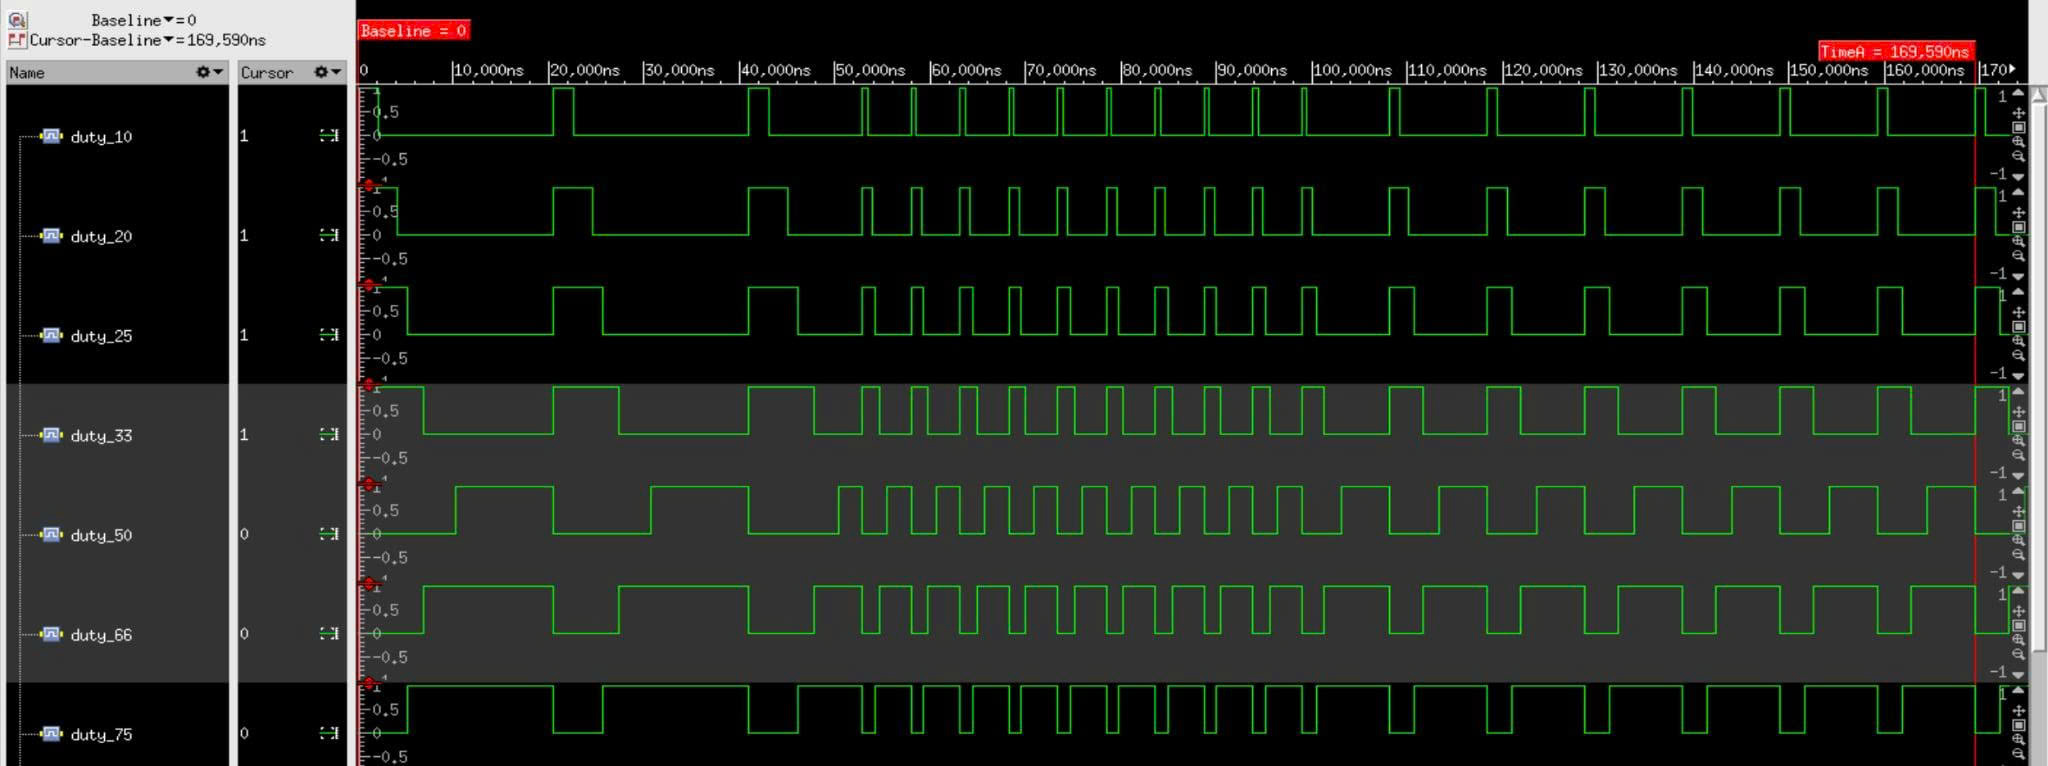
\includegraphics[width=.9\linewidth]{./my-chapters/my-images/simulation/duty_cycle.jpg}
	\caption{Demonstration of square waves with different duty cycles ranging from 10\% to 90\%.}
\end{figure}

\begin{figure}[H]
	\centering
	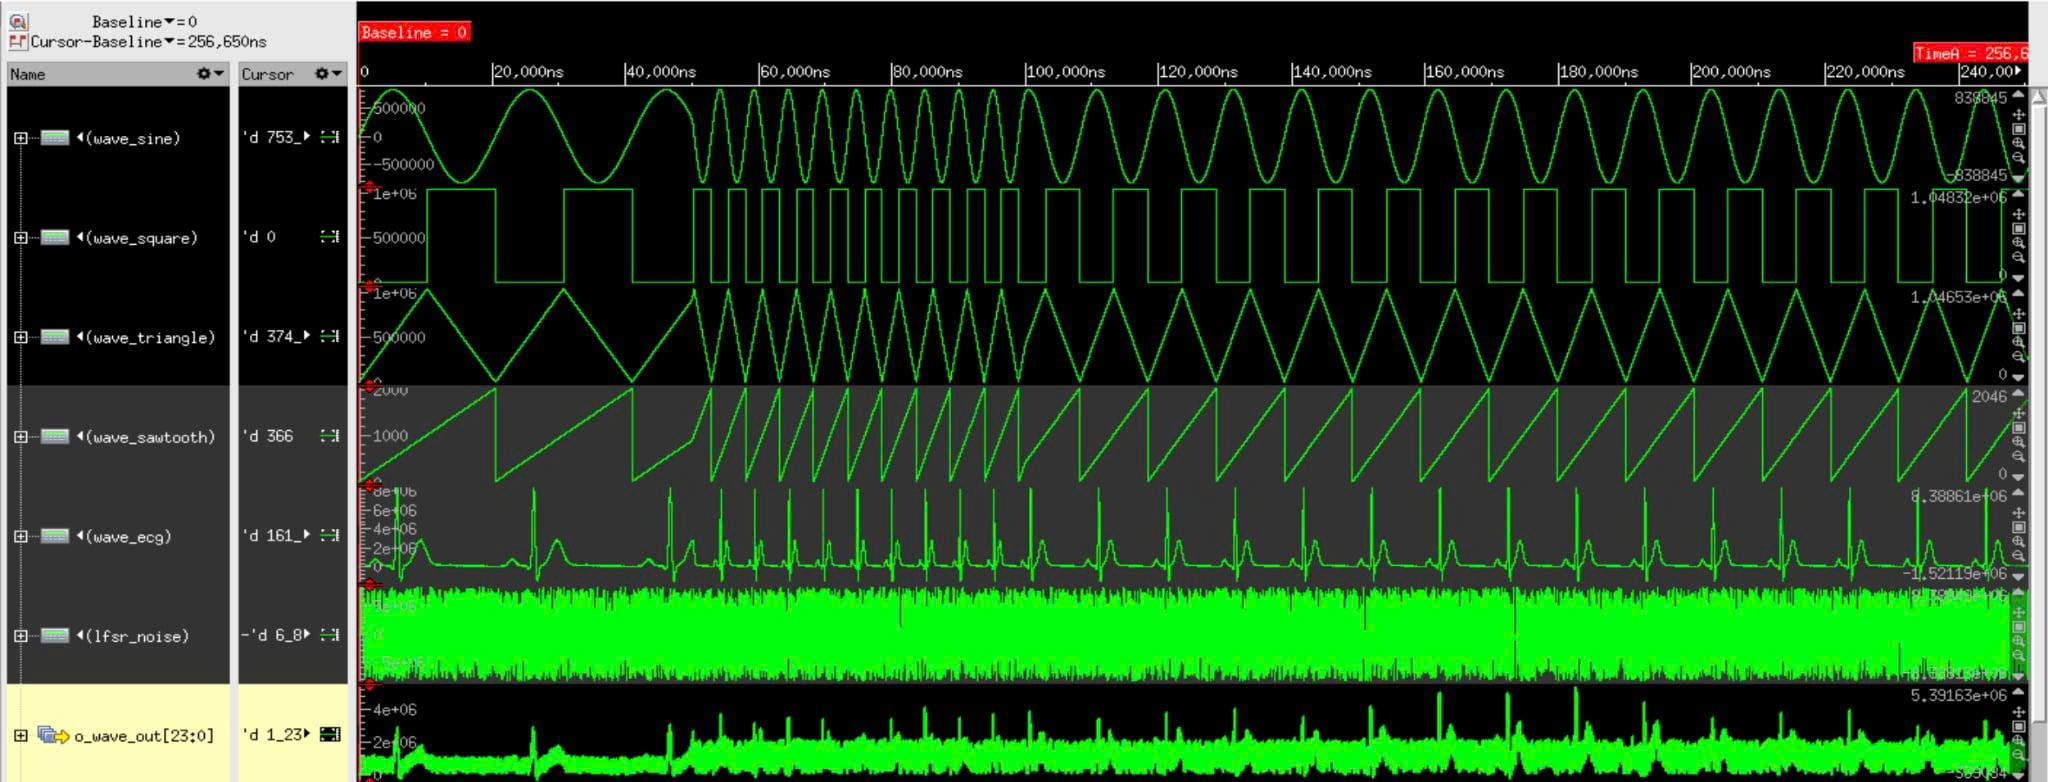
\includegraphics[width=.9\linewidth]{./my-chapters/my-images/simulation/waveform_with_noise.jpg}
	\caption{Basic waveforms and noise modulation: ECG output signal affected by frequency and amplitude variations of injected noise.}
\end{figure}

\subsection{Top module}

\begin{figure}[H]
	\centering
	\fbox{%
		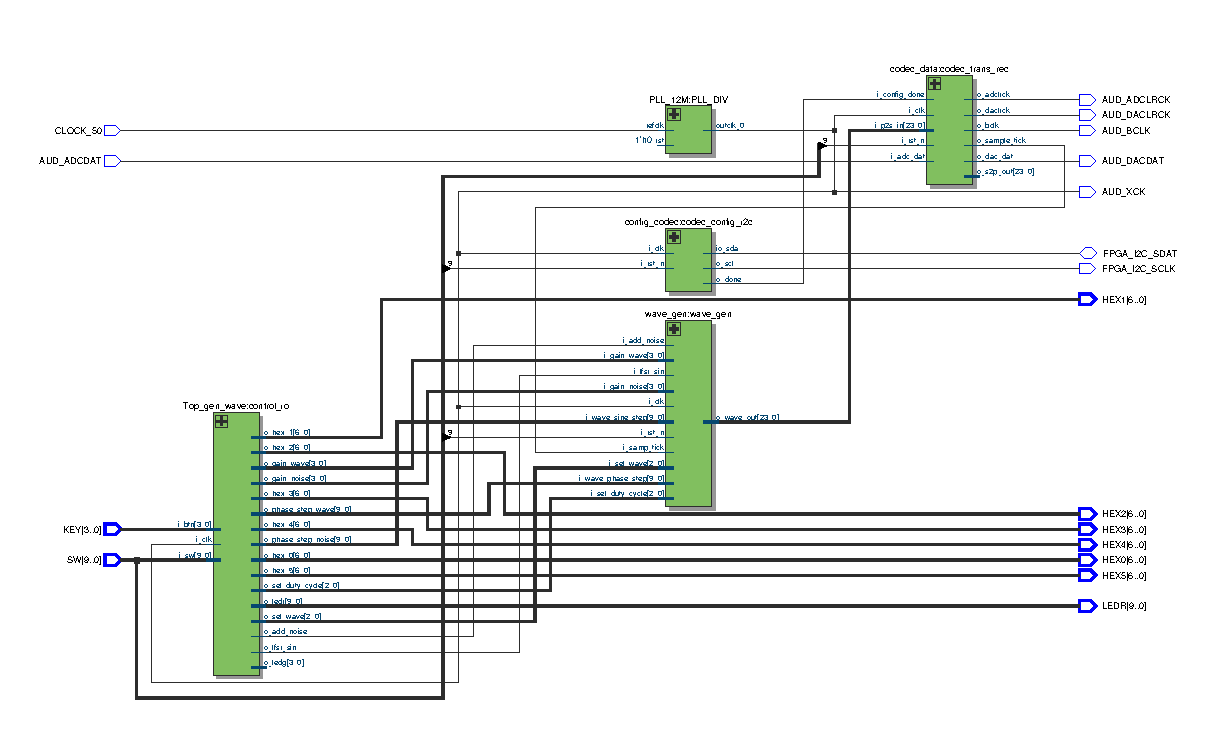
\includegraphics[width=\linewidth]{./my-chapters/my-diagrams/top_image.pdf}%
	}
	\caption{Block diagram for Top module.}
\end{figure}

\subsection{Measurement Waveform}

\begin{figure}[H]
	\centering
	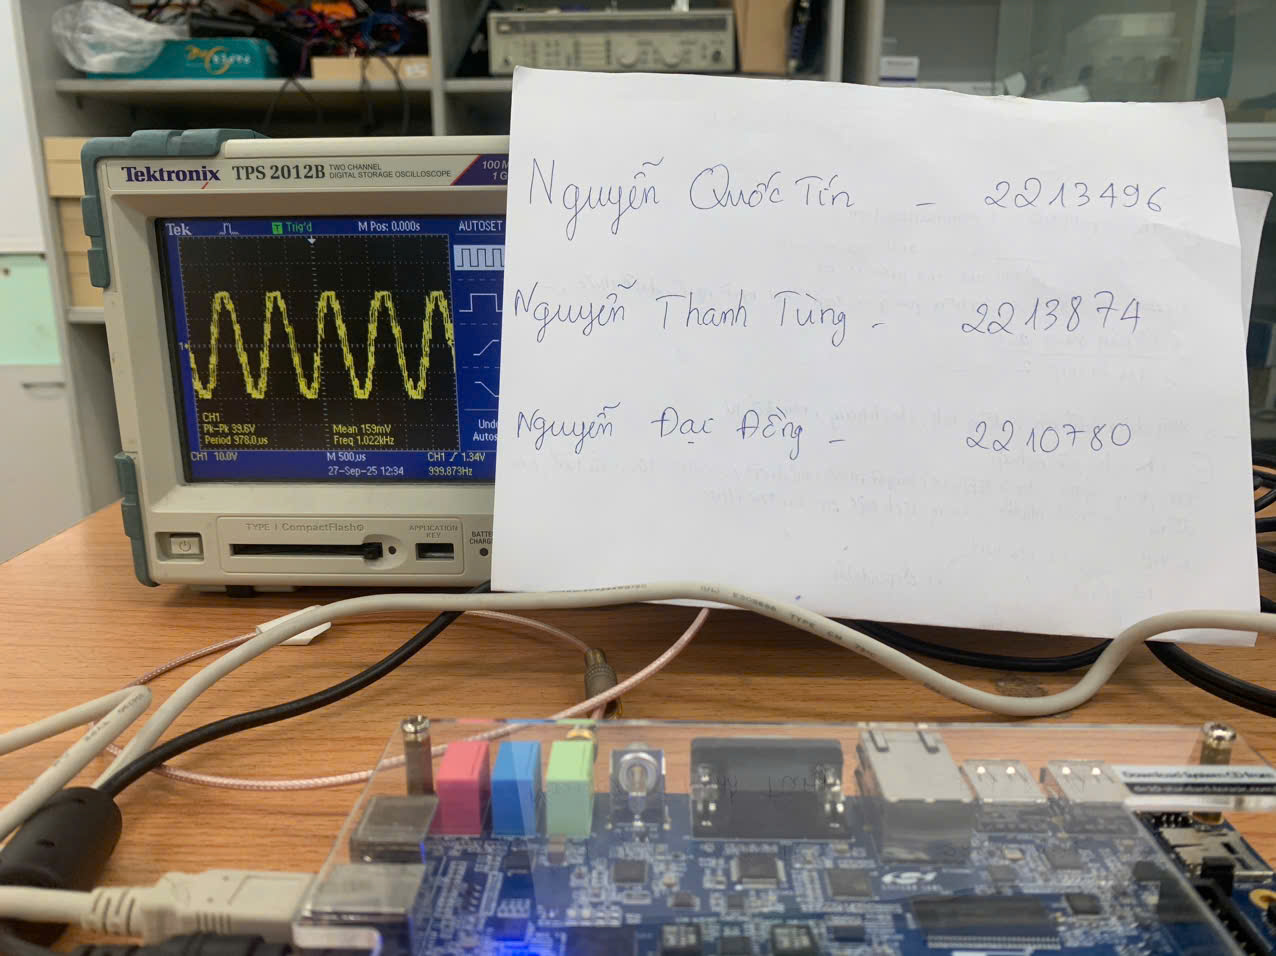
\includegraphics[width=.9\linewidth]{./my-chapters/my-images/Gen_wave/hinh2.jpg}
	\caption{Sine waveform on Oscilloscope.}
\end{figure}

\begin{figure}[H]
	\centering
	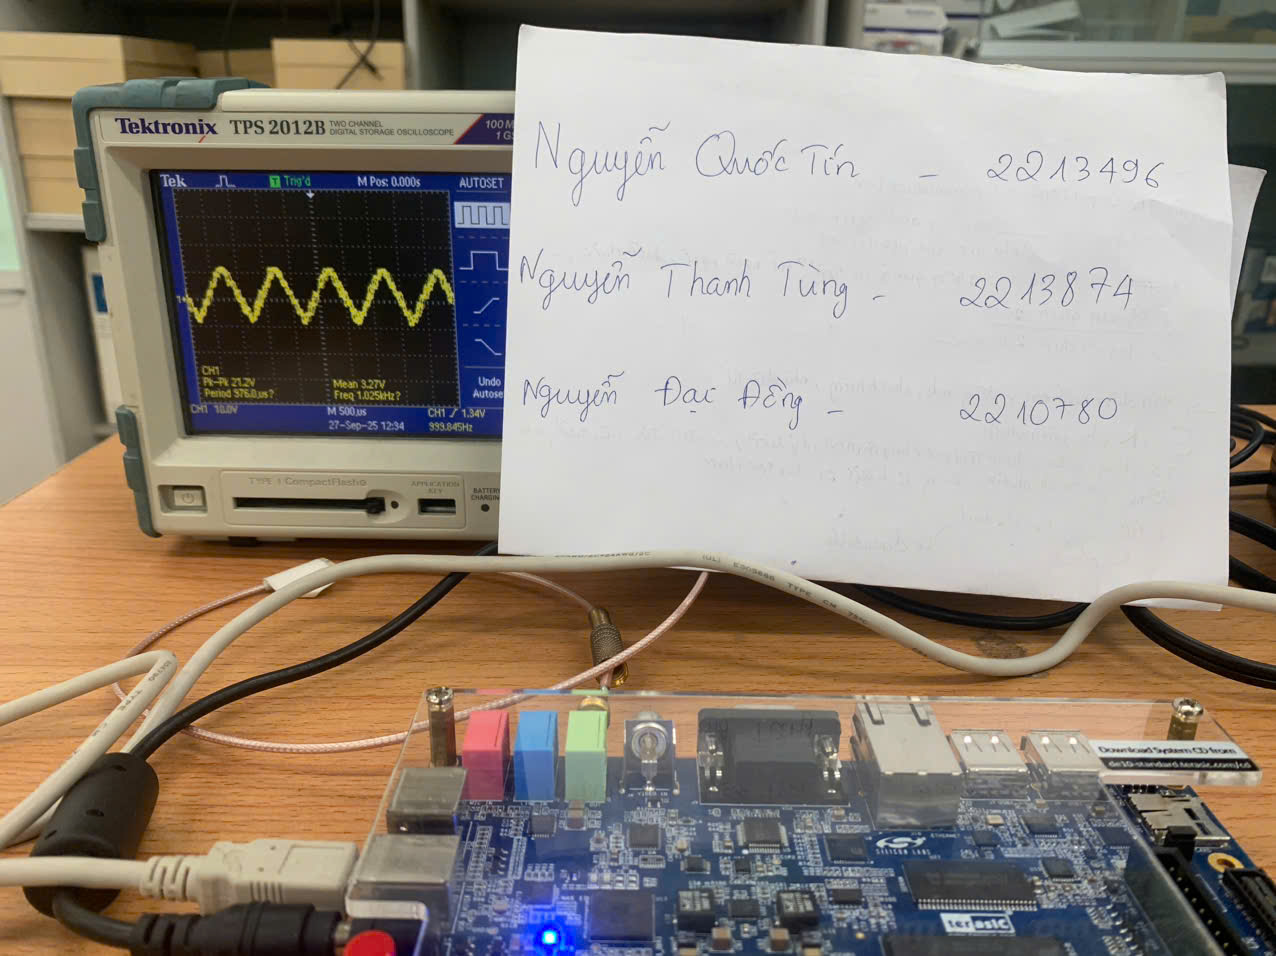
\includegraphics[width=.9\linewidth]{./my-chapters/my-images/Gen_wave/hinh5.jpg}
	\caption{Triangle waveform on Oscilloscope.}
\end{figure}

\begin{figure}[H]
	\centering
	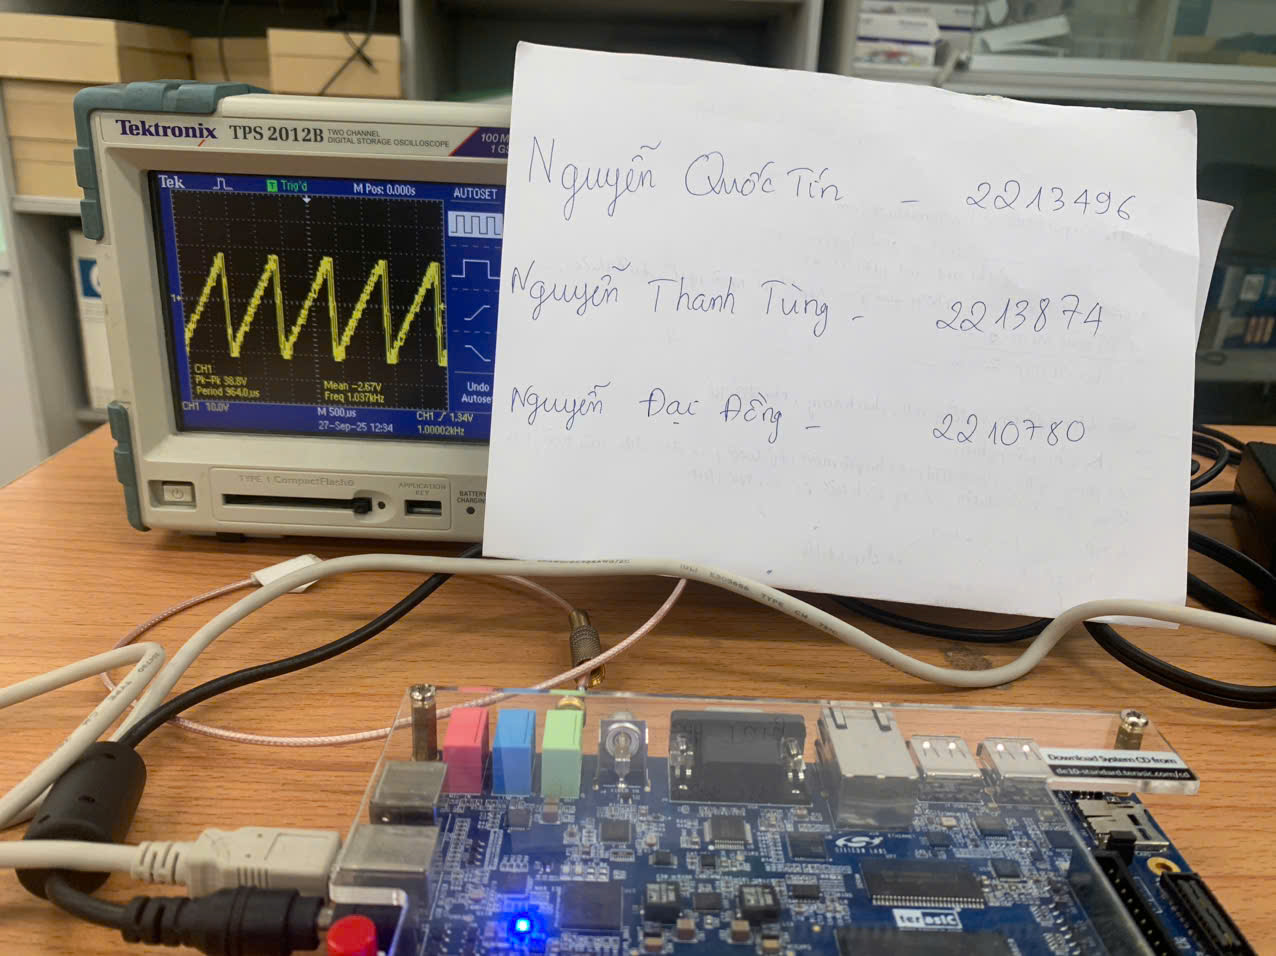
\includegraphics[width=.9\linewidth]{./my-chapters/my-images/Gen_wave/hinh4.jpg}
	\caption{Sawtooth waveform on Oscilloscope.}
\end{figure}

\begin{figure}[H]
	\centering
	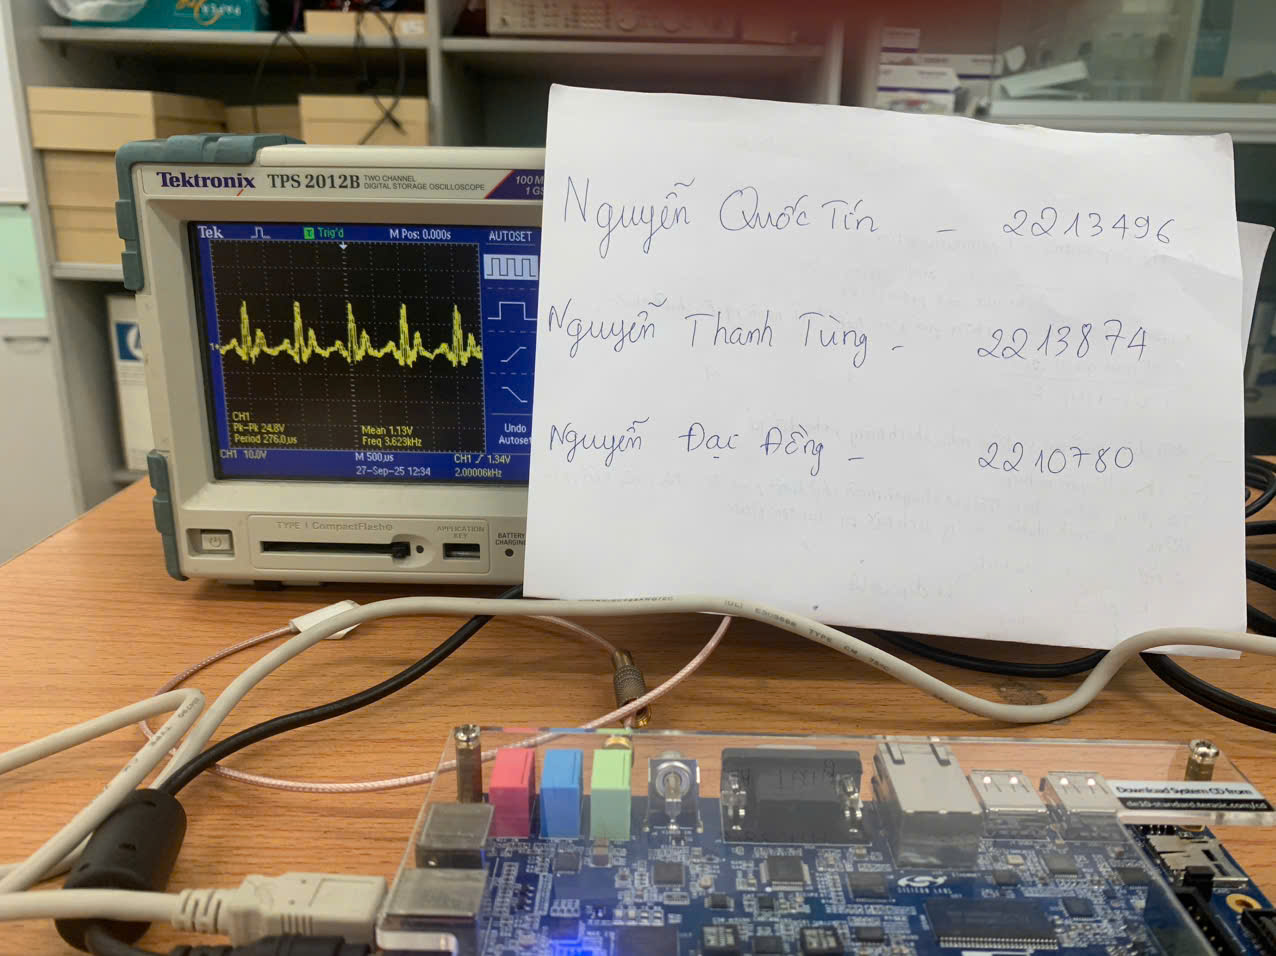
\includegraphics[width=.9\linewidth]{./my-chapters/my-images/Gen_wave/hinh3.jpg}
	\caption{ECG waveform on Oscilloscope.}
\end{figure}